\section{Background}\label{Background}

%
%  TAS / split tcp background
%  HF: Tim, I might have said wrong stuff here, please check
%

\subsection{TCP acceleration as a service (TAS)}

It is known that operating systems cause a large overhead on the network
stack. Arrakis \cite{peter:arrakis} showed that if we remove the kernel
from the packet processing path and do everything from user-level, the time 
required to process one packet can be up to 16 times less.

Because of this and network speeds ramping up, there has been plenty of work implementing
user-level network stacks \cite{mtcp, utcp, janus, alpine} with different ideas that try make general adoption
easier.

One of these ideas is TCP acceleration as a service (TAS or SplitTCP  ****TBD: check naming on intro/abstract***).
The idea behind TAS is that the TCP stack can be divided into two parts: a slow path, which does the connection
setup and teardown, and a fast path, where the data packets are sent and/or received. Figure \ref{fig:splittcp} 
shows the general idea of TAS; the user's application use an unmodified POSIX API to talk to a user-level TCP
library. The fast path can directly read from and write to the network card through DPDK \cite{dpdk}; when data packets
arrive or need to be sent out, the fast path directly communicates with the user-level library;
when it gets packets that have to be handled by the slow path (such as SYN packets), the packet 
is offloaded to it through shared memory. Because the two paths are executed in different threads, the slow path doesn't
affect the performance of the fast path.


\begin{figure}
\centering
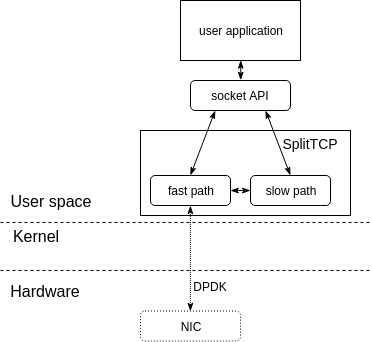
\includegraphics[width=0.7\columnwidth]{figures/splittcp_default.png}
\caption{The idea behind TAS is split network operations between a slow and a fast path, both in user level, completely
avoiding the kernel.}
\label{fig:splittcp}
\end{figure}


This idea yields very good performance for the average case of a datacenter: connections are long-lived and set up
pretty infrequently; thus data packets are predominant, making the fast path much more active than the slow path. One 
issue with this solution (and most other user-level stacks) is that all the desired kernel functionality are lost or
need to be reimplemented, such as
packet filtering, firewalls, control, etc.

%
% I couldn't glue both subsections, otherwise it would sound (even more) as an introduction
% so I just split them
%

\subsection{TAP devices}

One of the tools used in this work was TUN/TAP devices. These are virtual network devices that are purely software 
(hence the ``virtual''). These devices mimic a physical NIC, the only difference is that instead of receiving/sending
data to the outside through a wire/radio waves, it is done so to a buffer in kernel space that an application can read/write
through the POSIX file API. Figure \ref{fig:tap} has a basic representation of both concepts: when using a regular (wired)
NIC, the kernel gets calls from user space, and sends/receives from a physical device. When using a TUN/TAP device, the data is
read/written to a buffer in kernel, and an application in user space can capture and write raw network data to and from it, 
emulating a real outside connection.

The different between TUN and TAP is the network layer in which they work. TUN devices work in layer 3 (IP packets), while TAP
devices work in layer 2 (ethernet frames).


\begin{figure}
\centering
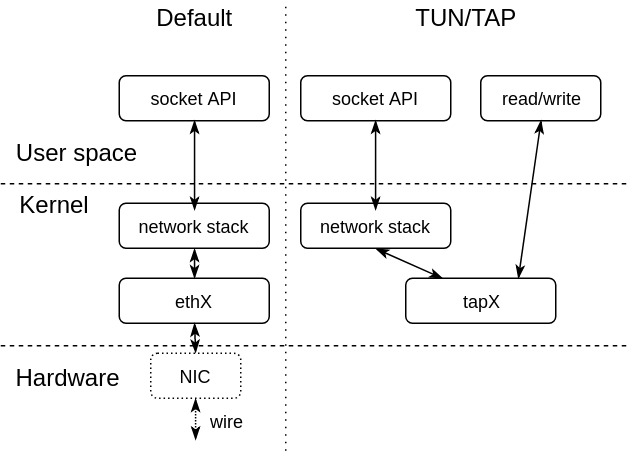
\includegraphics[width=0.7\columnwidth]{figures/tap_diag.png}
\caption{The difference between the usage of a regular NIC from a TUN/TAP device. In the latter the data is not sent to the
outside, but stored as raw data in a kernel space buffer which an application can read and write to.}
\label{fig:tap}
\end{figure}